% Copyright (c) 2026 Islam Ibrahim. All rights reserved.

\documentclass[tikz,border=16pt]{standalone}
\usepackage[T1]{fontenc}
\usepackage{amsmath,amssymb}
\usepackage{tikz}
\usetikzlibrary{arrows.meta, calc, positioning, patterns}

\begin{document}

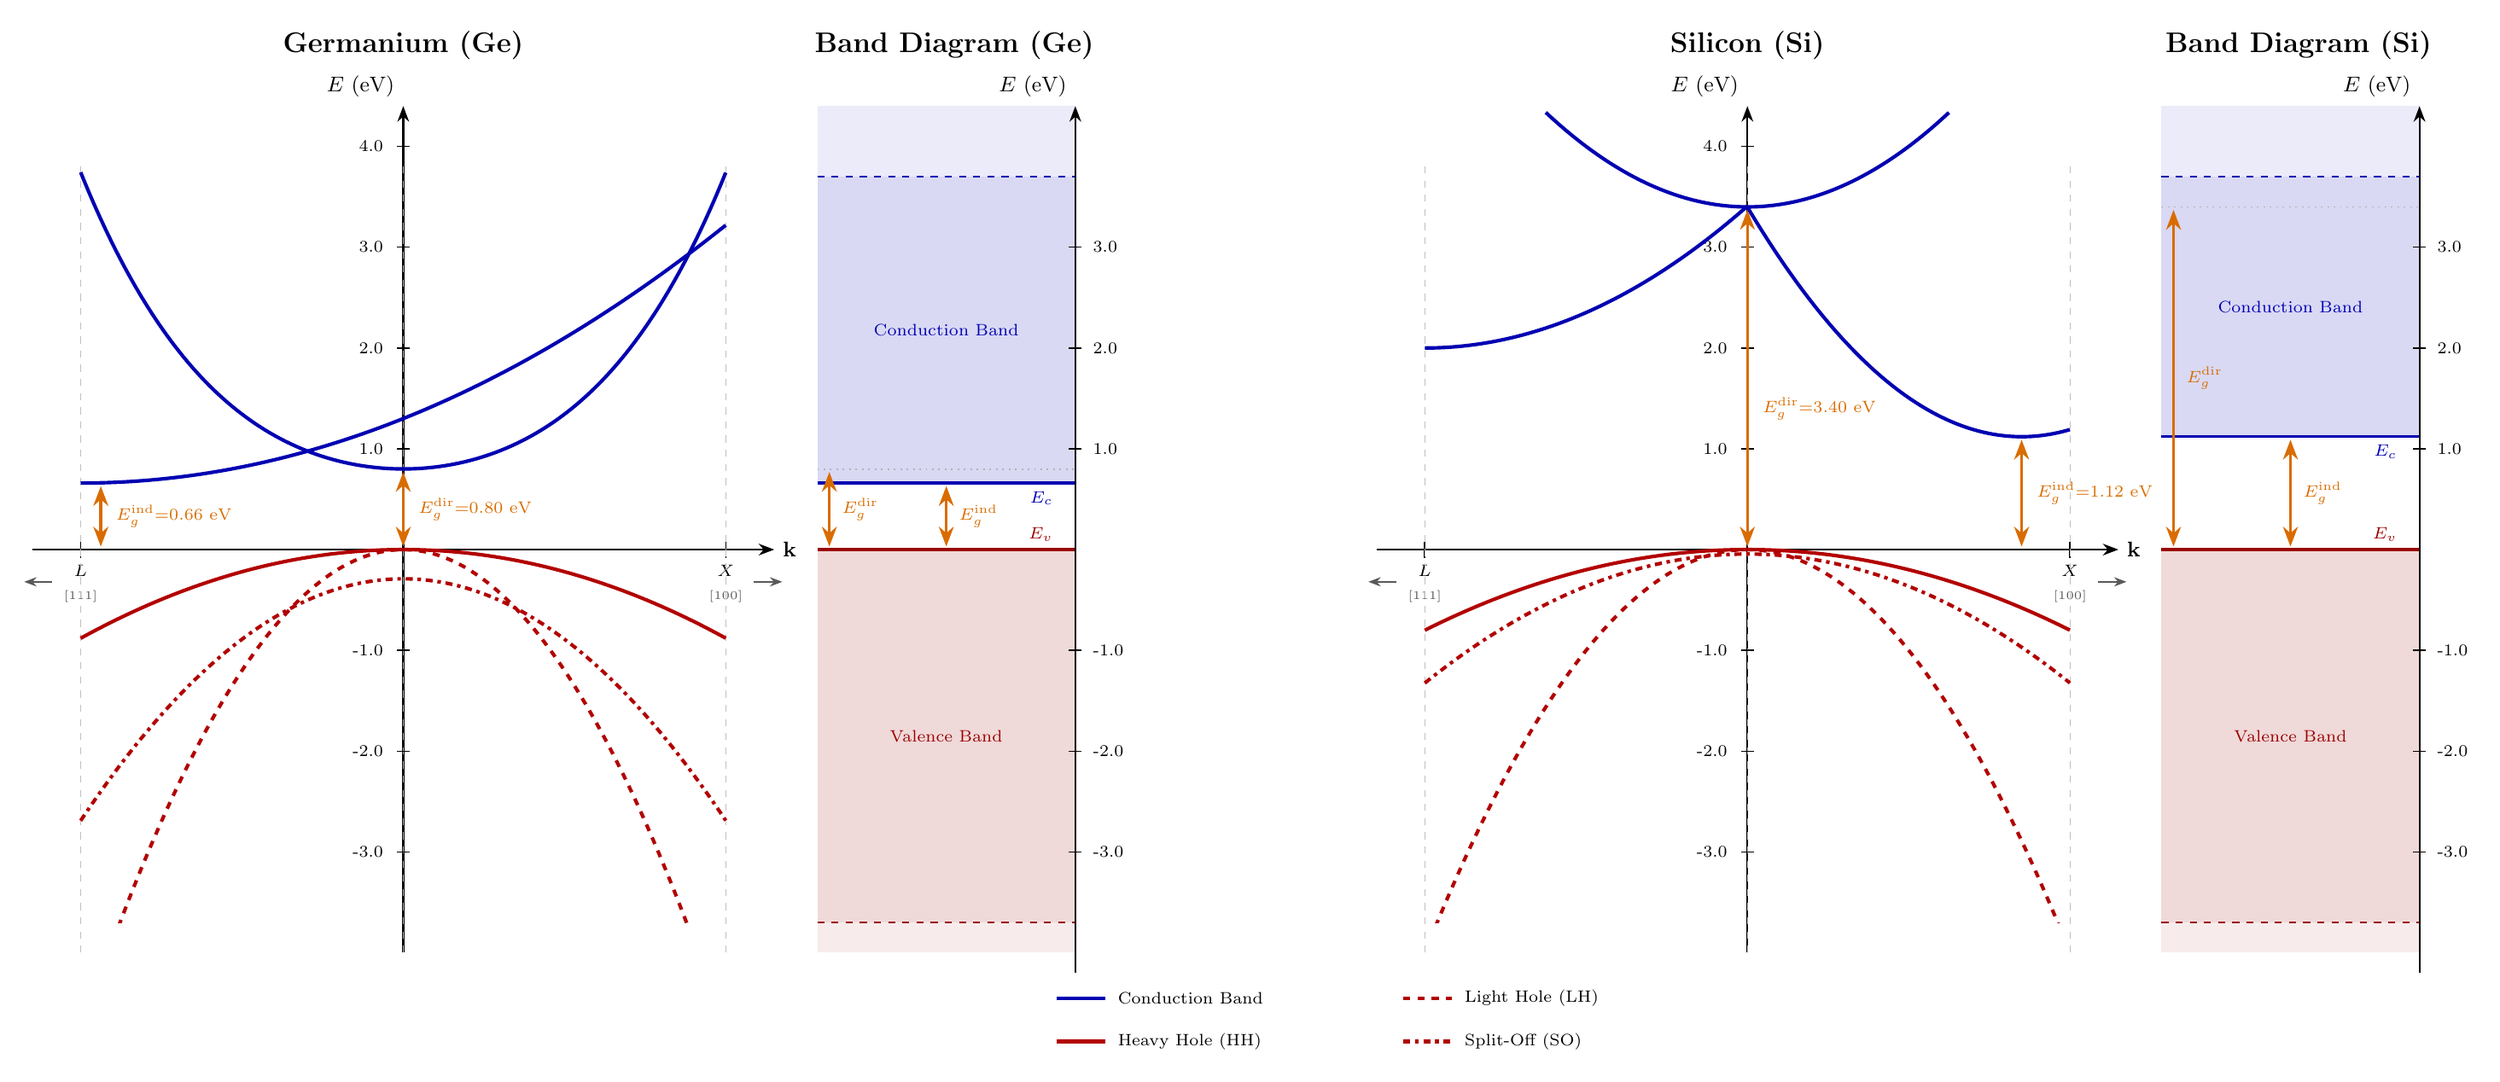
\begin{tikzpicture}[
  font=\small\rmfamily,
  >=Stealth,
  x=1.2cm, y=1.5cm,
  cb/.style   = {line width=1.5pt, blue!70!black},
  hh/.style   = {line width=1.5pt, red!70!black},
  lh/.style   = {line width=1.5pt, red!70!black, dashed},
  so/.style   = {line width=1.5pt, red!70!black, dash dot},
  egap/.style = {line width=1.2pt, orange!85!black, <->},
  guide/.style= {line width=0.4pt, gray!50, dashed},
  ann/.style  = {font=\small\rmfamily}
]

\def\kL{-4.0}
\def\kX{ 4.0}
\def\yBot{-4.0}
\def\yTop{4.4}
\def\yClip{-3.7}

\begin{scope}[xshift=0cm]
  \node[font=\large\bfseries] at (0, 5.0) {Germanium (Ge)};

  \draw[line width=0.8pt,->] (\kL-0.6,0) -- (\kX+0.6,0) node[right,ann] {$\mathbf{k}$};
  \draw[line width=0.8pt,->] (0,\yBot) -- (0,\yTop) node[above left,ann] {$E\ \text{(eV)}$};

  \draw[line width=0.6pt] (\kL,0.08) -- (\kL,-0.08);
  \node[ann, below=3pt, font=\scriptsize\rmfamily] at (\kL,0) {$L$};
  \node[ann, below=14pt, font=\tiny\rmfamily, gray!70!black] at (\kL,0) {$[111]$};
  \draw[<-, line width=0.5pt, gray!70!black] (\kL-0.7,-0.32) -- (\kL-0.35,-0.32);
  \draw[guide] (\kL,\yBot) -- (\kL,3.8);

  \draw[line width=0.6pt] (\kX,0.08) -- (\kX,-0.08);
  \node[ann, below=3pt, font=\scriptsize\rmfamily] at (\kX,0) {$X$};
  \node[ann, below=14pt, font=\tiny\rmfamily, gray!70!black] at (\kX,0) {$[100]$};
  \draw[->, line width=0.5pt, gray!70!black] (\kX+0.35,-0.32) -- (\kX+0.7,-0.32);
  \draw[guide] (\kX,\yBot) -- (\kX,3.8);

  \draw[line width=0.6pt] (0,0.08) -- (0,-0.08);
  \draw[guide] (0,\yBot) -- (0,3.8);

  \foreach \Ep in {4.0, 3.0, 2.0, 1.0, -1.0, -2.0, -3.0} {
    \draw[line width=0.5pt] (-0.08,\Ep) -- (0.08,\Ep);
    \node[ann, left=5pt, font=\scriptsize\rmfamily] at (0,\Ep) {\Ep};
  }

  \begin{scope}
    \clip (\kL-0.6, \yClip) rectangle (\kX+0.6, \yTop+0.2);
    \draw[cb] plot[domain=\kL:\kX, samples=150, smooth] (\x, { 0.66 + 0.04*(\x-\kL)^2 });
    \draw[cb] plot[domain=\kL:\kX, samples=150, smooth] (\x, { 0.80 + 0.12*(\x)^2 + 0.004*(\x)^4 });
    \draw[hh] plot[domain=\kL:\kX,samples=100,smooth] (\x, {-0.055*\x*\x});
    \draw[lh] plot[domain=\kL:\kX,samples=100,smooth] (\x, {-0.30*\x*\x});
    \draw[so] plot[domain=\kL:\kX,samples=100,smooth] (\x, {-0.290 - 0.15*\x*\x});
  \end{scope}

  \draw[egap] (\kL+0.25, 0.03) -- (\kL+0.25, 0.63);
  \node[ann, right=3pt, orange!85!black, font=\scriptsize\rmfamily]
      at (\kL+0.25, 0.33) {$E_{g}^{\mathrm{ind}}{=}0.66\ \mathrm{eV}$};

  \draw[egap] (0, 0.03) -- (0, 0.77);
  \node[ann, right=3pt, orange!85!black, font=\scriptsize\rmfamily]
      at (0, 0.40) {$E_{g}^{\mathrm{dir}}{=}0.80\ \mathrm{eV}$};
\end{scope}

\begin{scope}[xshift=10cm]
  \node[font=\large\bfseries] at (-1.5, 5.0) {Band Diagram (Ge)};

  \def\rectW{3.2}
  \def\GecbBot{0.66}
  \def\GecbDir{0.80}
  \def\GecbTop{3.70}
  \def\vbBot{-3.70}
  \def\vbTop{0.0}
  \def\axX{0.0}

  \fill[blue!70!black, opacity=0.15] (-\rectW, \GecbBot) rectangle (\axX, \GecbTop);
  \fill[blue!70!black, opacity=0.08] (-\rectW, \GecbTop) rectangle (\axX, \yTop);
  \draw[blue!70!black, line width=1.2pt] (-\rectW, \GecbBot) -- (\axX, \GecbBot);
  \draw[blue!70!black, line width=0.5pt, dashed] (-\rectW, \GecbTop) -- (\axX, \GecbTop);
  \node[font=\scriptsize\rmfamily, blue!70!black] at (-\rectW/2, {(\GecbBot+\GecbTop)/2}) {Conduction Band};

  \fill[red!60!black, opacity=0.15] (-\rectW, \vbBot) rectangle (\axX, \vbTop);
  \fill[red!60!black, opacity=0.08] (-\rectW, \vbBot) rectangle (\axX, \yBot);
  \draw[red!60!black, line width=1.2pt] (-\rectW, \vbTop) -- (\axX, \vbTop);
  \draw[red!60!black, line width=0.5pt, dashed] (-\rectW, \vbBot) -- (\axX, \vbBot);
  \node[font=\scriptsize\rmfamily, red!60!black] at (-\rectW/2, {(\vbBot+\vbTop)/2}) {Valence Band};

  \node[ann, left=6pt, font=\scriptsize\rmfamily, blue!70!black] at (\axX, \GecbBot-0.15) {$E_c$};
  \node[ann, left=6pt, font=\scriptsize\rmfamily, red!60!black]  at (\axX, \vbTop+0.15) {$E_v$};

  \draw[gray!60, line width=0.7pt, dotted] (-\rectW, \GecbDir) -- (\axX, \GecbDir);

  \draw[egap] (-\rectW+0.15, 0.03) -- (-\rectW+0.15, \GecbDir-0.03);
  \node[ann, right=2pt, orange!85!black, font=\scriptsize\rmfamily]
      at (-\rectW+0.15, \GecbDir/2) {$E_{g}^{\mathrm{dir}}$};

  \draw[egap] (-\rectW/2, 0.03) -- (-\rectW/2, \GecbBot-0.03);
  \node[ann, right=2pt, orange!85!black, font=\scriptsize\rmfamily]
      at (-\rectW/2, \GecbBot/2) {$E_{g}^{\mathrm{ind}}$};

  \draw[line width=0.8pt,->] (\axX, \yBot-0.2) -- (\axX, \yTop) node[above left, ann] {$E\ \text{(eV)}$};

  \foreach \Ep in {3.0, 2.0, 1.0, -1.0, -2.0, -3.0} {
    \draw[line width=0.5pt] (\axX-0.08,\Ep) -- (\axX+0.08,\Ep);
    \node[ann, right=4pt, font=\scriptsize\rmfamily] at (\axX,\Ep) {\Ep};
  }
\end{scope}

\begin{scope}[xshift=20cm]
  \node[font=\large\bfseries] at (0, 5.0) {Silicon (Si)};

  \draw[line width=0.8pt,->] (\kL-0.6,0) -- (\kX+0.6,0) node[right,ann] {$\mathbf{k}$};
  \draw[line width=0.8pt,->] (0,\yBot) -- (0,\yTop) node[above left,ann] {$E\ \text{(eV)}$};

  \draw[line width=0.6pt] (\kL,0.08) -- (\kL,-0.08);
  \node[ann, below=3pt, font=\scriptsize\rmfamily] at (\kL,0) {$L$};
  \node[ann, below=14pt, font=\tiny\rmfamily, gray!70!black] at (\kL,0) {$[111]$};
  \draw[<-, line width=0.5pt, gray!70!black] (\kL-0.7,-0.32) -- (\kL-0.35,-0.32);
  \draw[guide] (\kL,\yBot) -- (\kL,3.8);

  \draw[line width=0.6pt] (\kX,0.08) -- (\kX,-0.08);
  \node[ann, below=3pt, font=\scriptsize\rmfamily] at (\kX,0) {$X$};
  \node[ann, below=14pt, font=\tiny\rmfamily, gray!70!black] at (\kX,0) {$[100]$};
  \draw[->, line width=0.5pt, gray!70!black] (\kX+0.35,-0.32) -- (\kX+0.7,-0.32);
  \draw[guide] (\kX,\yBot) -- (\kX,3.8);

  \draw[line width=0.6pt] (0,0.08) -- (0,-0.08);
  \draw[guide] (0,\yBot) -- (0,3.8);

  \foreach \Ep in {4.0, 3.0, 2.0, 1.0, -1.0, -2.0, -3.0} {
    \draw[line width=0.5pt] (-0.08,\Ep) -- (0.08,\Ep);
    \node[ann, left=5pt, font=\scriptsize\rmfamily] at (0,\Ep) {\Ep};
  }

  \begin{scope}
    \clip (\kL-0.6, \yClip) rectangle (\kX+0.6, \yTop+0.2);
    \draw[cb] plot[domain=0:\kX, samples=100, smooth] (\x, { 1.12 + 0.197*(\x-3.4)^2 });
    \draw[cb] plot[domain=-2.5:2.5, samples=100, smooth] (\x, { 3.40 + 0.15*\x*\x });
    \draw[cb] plot[domain=\kL:0, samples=100, smooth] (\x, { 2.00 + 0.088*(\x-\kL)^2 });
    \draw[hh] plot[domain=\kL:\kX,samples=100,smooth] (\x, {-0.05*\x*\x});
    \draw[lh] plot[domain=\kL:\kX,samples=100,smooth] (\x, {-0.25*\x*\x});
    \draw[so] plot[domain=\kL:\kX,samples=100,smooth] (\x, {-0.044 - 0.08*\x*\x});
  \end{scope}

  \draw[egap] (3.4, 0.03) -- (3.4, 1.09);
  \node[ann, right=3pt, orange!85!black, font=\scriptsize\rmfamily]
      at (3.4, 0.56) {$E_{g}^{\mathrm{ind}}{=}1.12\ \mathrm{eV}$};

  \draw[egap] (0, 0.03) -- (0, 3.37);
  \node[ann, right=3pt, orange!85!black, font=\scriptsize\rmfamily]
      at (0, 1.40) {$E_{g}^{\mathrm{dir}}{=}3.40\ \mathrm{eV}$};
\end{scope}

\begin{scope}[xshift=30cm]
  \node[font=\large\bfseries] at (-1.5, 5.0) {Band Diagram (Si)};

  \def\rectW{3.2}
  \def\SicbBot{1.12}
  \def\SicbDir{3.40}
  \def\SicbTop{3.70}
  \def\vbBot{-3.70}
  \def\vbTop{0.0}
  \def\axX{0.0}

  \fill[blue!70!black, opacity=0.15] (-\rectW, \SicbBot) rectangle (\axX, \SicbTop);
  \fill[blue!70!black, opacity=0.08] (-\rectW, \SicbTop) rectangle (\axX, \yTop);
  \draw[blue!70!black, line width=1.2pt] (-\rectW, \SicbBot) -- (\axX, \SicbBot);
  \draw[blue!70!black, line width=0.5pt, dashed] (-\rectW, \SicbTop) -- (\axX, \SicbTop);
  \node[font=\scriptsize\rmfamily, blue!70!black] at (-\rectW/2, {(\SicbBot+\SicbTop)/2}) {Conduction Band};

  \fill[red!60!black, opacity=0.15] (-\rectW, \vbBot) rectangle (\axX, \vbTop);
  \fill[red!60!black, opacity=0.08] (-\rectW, \vbBot) rectangle (\axX, \yBot);
  \draw[red!60!black, line width=1.2pt] (-\rectW, \vbTop) -- (\axX, \vbTop);
  \draw[red!60!black, line width=0.5pt, dashed] (-\rectW, \vbBot) -- (\axX, \vbBot);
  \node[font=\scriptsize\rmfamily, red!60!black] at (-\rectW/2, {(\vbBot+\vbTop)/2}) {Valence Band};

  \node[ann, left=6pt, font=\scriptsize\rmfamily, blue!70!black] at (\axX, \SicbBot-0.15) {$E_c$};
  \node[ann, left=6pt, font=\scriptsize\rmfamily, red!60!black]  at (\axX, \vbTop+0.15) {$E_v$};

  \draw[gray!60, line width=0.7pt, dotted] (-\rectW, \SicbDir) -- (\axX, \SicbDir);

  \draw[egap] (-\rectW+0.15, 0.03) -- (-\rectW+0.15, \SicbDir-0.03);
  \node[ann, right=2pt, orange!85!black, font=\scriptsize\rmfamily]
      at (-\rectW+0.15, \SicbDir/2) {$E_{g}^{\mathrm{dir}}$};

  \draw[egap] (-\rectW/2, 0.03) -- (-\rectW/2, \SicbBot-0.03);
  \node[ann, right=2pt, orange!85!black, font=\scriptsize\rmfamily]
      at (-\rectW/2, \SicbBot/2) {$E_{g}^{\mathrm{ind}}$};

  \draw[line width=0.8pt,->] (\axX, \yBot-0.2) -- (\axX, \yTop) node[above left, ann] {$E\ \text{(eV)}$};

  \foreach \Ep in {3.0, 2.0, 1.0, -1.0, -2.0, -3.0} {
    \draw[line width=0.5pt] (\axX-0.08,\Ep) -- (\axX+0.08,\Ep);
    \node[ann, right=4pt, font=\scriptsize\rmfamily] at (\axX,\Ep) {\Ep};
  }
\end{scope}

\begin{scope}[xshift=0cm]
  \draw[cb] (8.1, -4.45) -- (8.7, -4.45);
  \node[ann, right=2pt, font=\scriptsize\rmfamily] at (8.7, -4.45) {Conduction Band};
  \draw[hh] (8.1, -4.88) -- (8.7, -4.88);
  \node[ann, right=2pt, font=\scriptsize\rmfamily] at (8.7, -4.88) {Heavy Hole (HH)};

  \draw[lh] (12.4, -4.45) -- (13.0, -4.45);
  \node[ann, right=2pt, font=\scriptsize\rmfamily] at (13.0, -4.45) {Light Hole (LH)};
  \draw[so] (12.4, -4.88) -- (13.0, -4.88);
  \node[ann, right=2pt, font=\scriptsize\rmfamily] at (13.0, -4.88) {Split-Off (SO)};
\end{scope}

\end{tikzpicture}

\end{document}